\section*{研究方法论述}

本提案的主要研究成果围绕三个阶段展开: \textbf{(1) 数据准备}、 \textbf{(2) 模型开发}、 and \textbf{(3) 实际应用测试。}


\subsection*{阶段一数据准备与特征工程}
本阶段专注于为模型训练准备和组织数据。它涉及收集每个语言的多样化高质量音频语料库,涵盖各种说话者、年龄和情绪。必要的标注将包含说话者特征、表达的情绪以及对应的文本。语料库的设计将涵盖每种语言内的各种口音、方言和说话风格。将收集特定于不同媒体(例如有声读物、有声剧、纪录片)的平行语料库(音频和相应的脚本),以捕捉语境差异。数据将通过降噪、归一化和将语音分割成单独的单元等方法进行预处理,以解决不一致问题并提高整体质量。自动和手动特征提取程序将识别相关的声学线索(例如音高、能量、频谱特征)和语言特征(例如音素持续时间、停顿持续时间、声调变化、韵律轮廓),这些特征对于建模语言特定的韵律至关重要。提取的特征将以适合模型架构的方式进行精细化表示。

\subsection*{阶段二模型开发与训练}
本阶段将设计一个基于Transformer架构的新型多语言TTS框架。该框架将整合多模态编码器,以整合语言信息、说话人特征和情感线索。该架构将包含语言特定组件,以处理每种语言(英语、孟加拉语和中文)的独特韵律和语音特征。该框架将使用合适的优化技术和损失函数在准备好的语料库上进行训练。将使用保留数据进行严格验证,以评估框架的泛化能力。在训练过程中持续使用相关指标(如MOS)进行评估,将指导模型的开发和改进。本阶段重点在于迭代模型改进和超参数优化,这些优化将由性能评估指导。

\subsection*{ 阶段三实际应用测试与评估}
本阶段评估所开发框架的实际可用性。训练后的模型将被调整以适应特定的实际应用(例如,为有声读物、有声剧和纪录片生成音频)。将设计用户友好的界面,以实现潜在的部署。将进行全面的评估,结合客观指标(平均意见得分、ASR 错误率)和专家小组(配音演员、语言学家和音频专业人士)的主观评估,以评估该框架在每个应用情境中的有效性和整体质量。该评估将重点关注合成语音的自然度、表达性和文化恰当性,为迭代改进提供关键反馈。

\begin{center}
    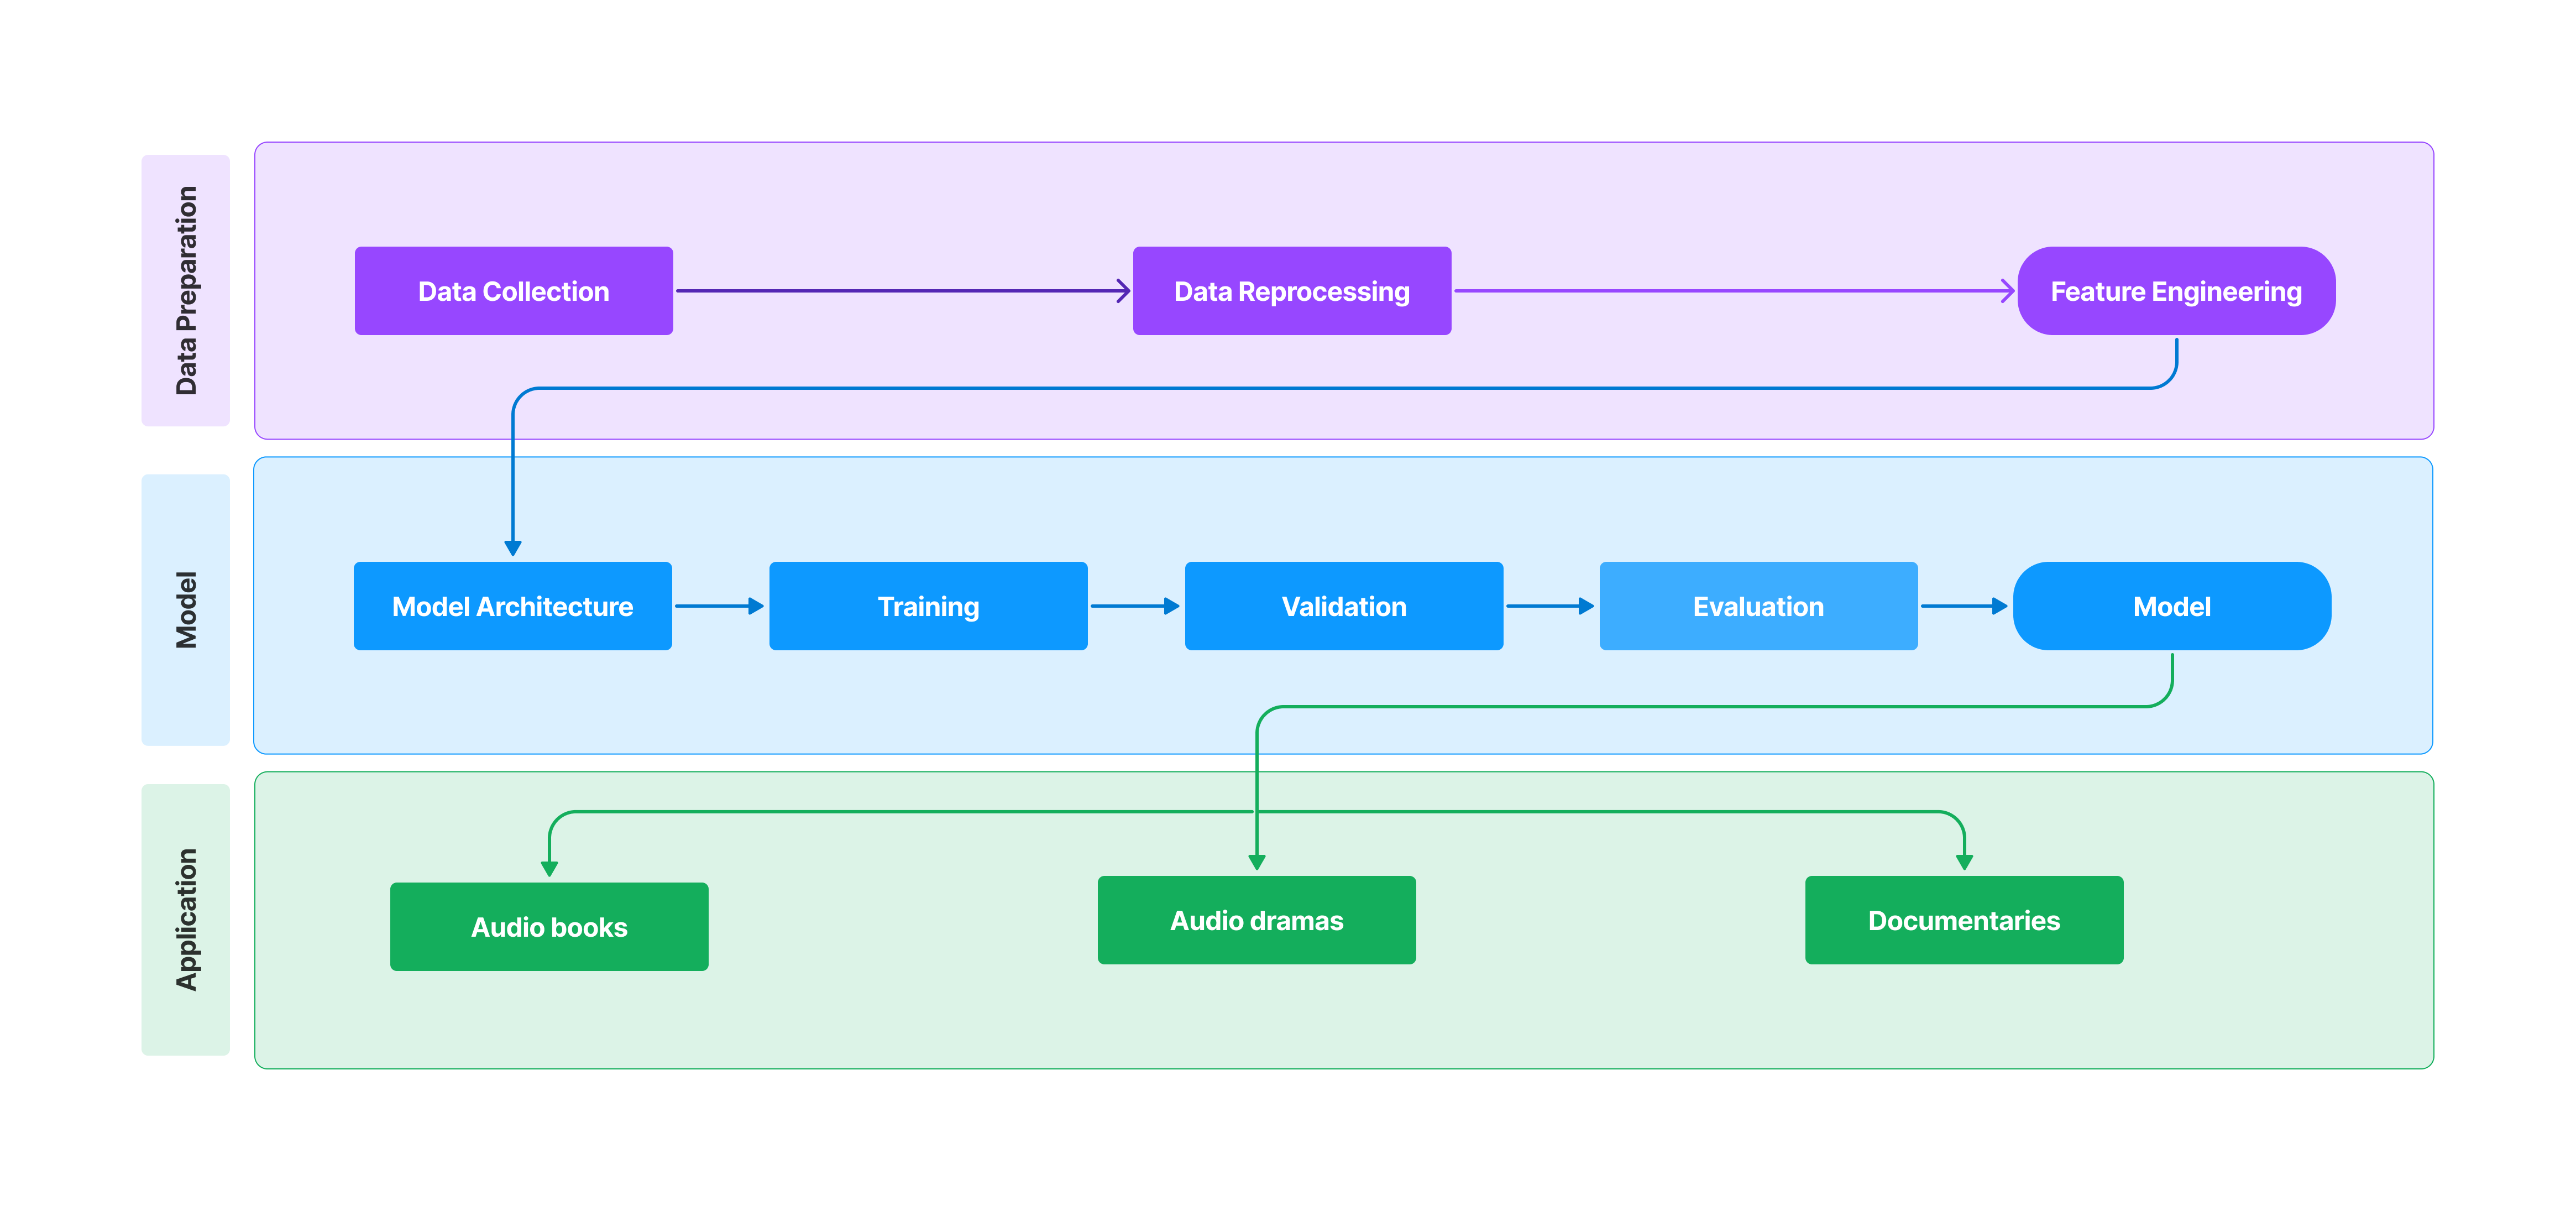
\includegraphics[width=1.0\textwidth]{research-flow.png}
    \captionof{figure}{Research flow}
\end{center}

该方法采用分阶段的方法开发一个强大的多语言TTS框架。数据准备、模型开发和实际应用测试阶段确保了全面的评估,并使该框架适合于有声读物和纪录片等应用。该方法优先考虑多样化数据、语言特定建模和专家评估,以创建高质量且实用的系统。